\documentclass{article}
\usepackage{geometry}
\usepackage{amsmath}
% \usepackage{ctex}
\usepackage{amsmath,amsfonts,amssymb,epsfig,graphicx}
\usepackage{tabularx}
\usepackage{booktabs}
\usepackage{arydshln}
\usepackage{color}

\geometry{ left=1in, right=2in, top=1in, bottom=1in}
\setlength{\marginparwidth}{1.5in}
\newcommand{\ket}[1]{\left|#1\right\rangle}
\newcommand{\bra}[1]{\left\langle#1\right|}
\newcommand{\braket}[1]{\left\langle#1\right\rangle}
% \newcommand{\average}[1]{\left\langle#1\right\rangle}
\begin{document}
\title{Research Note - Quantum Entanglement}
\author{Youpeng Wu}
\date{\today}
\maketitle

\section{Basical Concepts }
\subsection{Density matrix}
As defination of density matrix, for a quantum complete set of states \(\{\ket{n}\}\) which satisfy \(\sum_n \ket{n}\bra{n}=1\), the density matrix is:
\[\rho=\ket{n}\bra{n}\]
and it's trace is \(\mathrm{tr}\ \rho=1\). It can be used to caculate the average value of an observable \(G\)\marginpar{Funny fact: \[\nabla\cdot A\vec{x}=\mathrm{tr}(A)\]}: 
\[\braket{G}=\braket{\psi|G|\psi}=\sum_{n,n^\prime}\braket{\psi|n}\braket{n|G|n^\prime}\braket{n^\prime|\psi}=\mathrm{tr}(\rho G)\]
If quantum state cannot be described by ONE wave function, in other words, the quantum state is a mixed state\(\ket{\psi}=\sum_k c_k\ket{k}=\sum_kp_k\ket{k},\sum_k p_k=1\), the density matrix is:
\[\rho=\sum_k p_k\ket{k}\bra{k}\]

\subsection{Irreducible tensor}


\subsection{\(SU(3)\) symmetry matrix}
For a \(SU(3)\) symmetry matrix, the matrix\(\lambda_i\) is:
\begin{table}[htb]
    \caption{Gell-Mann matrix}
    \label{tab:gmmatrix}
    \centering
    \begin{tabularx}{0.75\textwidth}{c|c|c}
        \toprule
        \(\lambda_1=\begin{bmatrix}0 & 1 & 0\\1 & 0 & 0\\ 0 & 0 & 0 \end{bmatrix}\) &
        \(\lambda_2=\begin{bmatrix}0 & -i & 0\\i & 0 & 0\\ 0 & 0 & 0 \end{bmatrix}\) &
        \(\lambda_3=\begin{bmatrix}1 & 0 & 0\\0 & -1 & 0\\ 0 & 0 & 0 \end{bmatrix}\) \\
        \midrule
        \(\lambda_4=\begin{bmatrix}0 & 0 & 1\\0 & 0 & 0\\ 1 & 0 & 0 \end{bmatrix}\) &
        \(\lambda_5=\begin{bmatrix}0 & 0 & -i\\0 & 0 & 0\\ i & 0 & 0 \end{bmatrix}\) &
        \(\lambda_6=\begin{bmatrix}0 & 0 & 0\\0 & 0 & 1\\ 0 & 1 & 0 \end{bmatrix}\) \\
        \midrule
        \(\lambda_7=\begin{bmatrix}0 & 0 & 0\\0 & 0 & -i\\ 0 & i & 0 \end{bmatrix}\) &
        \(\lambda_8=\frac{1}{\sqrt{3}}\begin{bmatrix}1 & 0 & 0\\0 & 1 & 0\\ 0 & 0 & -2 \end{bmatrix}\) &
        - \\
        \bottomrule
    \end{tabularx}
\end{table}
we define transformation matrix \(U\) as:
\[\phi^\prime=U\phi\]
which:
\[U=\exp\left[\frac{1}{2}i\hat{\theta}\hat{n}\cdot\lambda\right]\]

\section{Bell inequalities}
\subsection{CHSH inequality derivation}

The proof\cite{clauser1974experimental} of the CHSH inequality is based on the following assumptions: \textbf{Local hidden variable} theories: the measurement results of the two particles are determined by the hidden variables of the particles themselves, and the measurement results of the two particles are independent of each other.

We assume there a pair of entangled particles for \(a\), \(a^\prime\), \(b\), \(b^\prime\) are different measurement directions, and \(A\), \(A^\prime\), \(B\), \(B^\prime\) are the measurement results which's possibe value are \(\{-1,0,1\}\). In other words, \(A\) are observables in \(\mathcal{H}_A\), and \(B\) are observables in \(\mathcal{H}_B\). If the local hidden variable theories are correct, the possiblity of pairs of outcomes \(P(a,b)\) is: 
\[P(a,b)=\int d\lambda A(a,\lambda) B(b,\lambda) \rho(\lambda) \]
where \(\lambda\) is the hidden variable, and \(\rho(\lambda)\) is the probability distribution of the hidden variable. So that:
\begin{align*}
    &P(a,b)-P(a,b^\prime)\\
    &=\int d\lambda \rho(\lambda) [A(a,\lambda)B(b,\lambda)-A(a,\lambda)B(b^\prime,\lambda)]\\
    &=\int d\lambda \rho(\lambda) [A(a,\lambda)B(b,\lambda)-A(a,\lambda)B(b^\prime,\lambda)\pm A(a,\lambda)B(b^\prime,\lambda)A(a^\prime,\lambda)B(b^\prime,\lambda)\mp A(a,\lambda)B(b^\prime,\lambda)A(a^\prime,\lambda)B(b^\prime,\lambda) ] \\
    &=\int d\lambda \rho(\lambda) A(a,\lambda) B(b,\lambda)[1\pm A(a^\prime,\lambda)B(b^\prime,\lambda)]-A(a,\lambda)B(b^\prime,\lambda)[1\pm A(a^\prime,\lambda)B(b,\lambda)]
\end{align*}
apply the triangle inequality  (\(c=a+b\Rightarrow|c|\leqslant |a|+|b|\)):
\begin{align*}
    &|P(a,b)-P(a,b^\prime)|\\
    &\leqslant \left|\int d\lambda \rho(\lambda) A(a,\lambda) B(b,\lambda)[1\pm A(a^\prime,\lambda)B(b^\prime,\lambda)]\right|+\left|\int d\lambda \rho(\lambda) A(a,\lambda)B(b^\prime,\lambda)[1\pm A(a^\prime,\lambda)B(b,\lambda)]\right|\\
    &\leqslant \int d\lambda \left|A(a,\lambda) B(b,\lambda)\right|\left|1\pm A(a^\prime,\lambda)B(b^\prime,\lambda)\right|+\int d\lambda \left|A(a,\lambda)B(b^\prime,\lambda)\right|\left|1\pm A(a^\prime,\lambda)B(b,\lambda)\right|\\
\end{align*}
cause \([1\pm A(a^\prime,\lambda)B(b^\prime,\lambda)]\rho(\lambda) \geqslant 0 \), and \([1\pm A(a^\prime,\lambda)B(b,\lambda)]\rho(\lambda) \geqslant 0 \) they are \textbf{non-negative}. \marginpar{Because both A, B, A', B' are \(\{-1,0,1\}\), the absolute value of the product of them is 1.} Then we have:
\begin{align*}
    &|P(a,b)-P(a,b^\prime)|\\
    &\leqslant \int d\lambda \rho(\lambda) [1\pm A(a^\prime,\lambda)B(b^\prime,\lambda)]+\int d\lambda \rho(\lambda) [1\pm A(a^\prime,\lambda)B(b,\lambda)]\\
    &\leqslant 2 \pm \left[\int d\lambda \rho(\lambda) A(a^\prime,\lambda)B(b^\prime,\lambda) + \int d\lambda \rho(\lambda) A(a^\prime,\lambda)B(b,\lambda)\right]\\
    &\leqslant 2 \pm \left[P(a^\prime,b^\prime)+P(a^\prime,b)\right]
\end{align*}
where the last inequality is the definition of \(P(a^\prime,b^\prime)\) and \(P(a^\prime,b)\). So that\marginpar{We use triangle inequality again}:
\begin{align*}
    &|P(a,b)-P(a,b^\prime)|\leqslant 2 \pm \left[P(a^\prime,b^\prime)+P(a^\prime,b)\right]\\
    &\Rightarrow |P(a,b)-P(a,b^\prime)|+|P(a,b)+P(a,b^\prime)|\leqslant 2\\
    &\Rightarrow |P(a,b)-P(a,b^\prime)+P(a,b)+P(a,b^\prime)|\leqslant \text{Left.} \leqslant 2
\end{align*}
Q.E.D. 

But for the quantum mechanics, the measurement results of the two particles are not independent of each other, so that the CHSH inequality is violated. for two particles with spin \(1\), the state of particles is: \(\{\ket{+},\ket{0},\ket{-}\}\), so pair of particles are in the state:
\[\{\ket{+},\ket{0},\ket{-}\}_A\otimes\{\ket{+},\ket{0},\ket{-}\}_B\]
Cause limit of spin momentum conservation, the state of the two particles must be:
\[\ket{\psi_{s}}=\frac{1}{\sqrt{3}}(\ket{+-}-\ket{00}+\ket{-+})\]


\subsection{CGLMP inequality}
Our measurement is based on 3 dimension (spin 1)In Spin-1 case (3 dimension), the density matrix\marginpar{Detiel of proof in ~\cite{fabbrichesi_bell_2023} section 2.3}
%[TODO] add density matrix of spin 1

For pherhaps of local hidden variable theories, CGLMP inequality\cite{dalton2021cglmp}, in the case of two particles with spin \(1\), the inequality\cite{Collins_2002} is:
\begin{align*}
    I_3\leq &2 \\
    \textrm{which:}\quad I_3 = &+[P(A_1=B_1)+P(B_1=A_2+1)\\
          &+P(A_2=B_2)+P(B_2=A_1)]\\
          &-[P(A_1=B_1-1)+P(B_1=A_2)\\
          &+P(A_2=B_2-1)+P(B_2=A_1-1)]
\end{align*}
where \(A_i\) and \(B_i\) are the measurement results of the two particles, and \(P(A_i=B_j)\) is the probability of the two particles having the same measurement results. We can use Bell operator \(\mathcal{O}_{Bell}\) for the inequality:
\[I_3=\braket{\mathcal{O}_{Bell}}=\mathrm{tr}\{\rho \mathcal{O}_{Bell} \}\leqslant 2\]

For our \(H\rightarrow ZZ\) process, \(ZZ\) state must be:
\[\ket{\psi_{ZZ}}=a_1\ket{+-}+a_2\ket{00}+a_3\ket{-+}\]
where \(a_1^2+a_2^2+a_3^2=1\). 
\[e_\sigma^\mu(m,\vec{k})=\begin{array}{c:c}
	\,\, &		{\color[RGB]{0,0,255}\begin{matrix}
	S_-&	\quad S_0&		\quad S_0\\
\end{matrix}}\\\hdashline{\color[RGB]{0, 0, 255} \begin{array}{c}k_0\\k_x\\k_y\\k_z\\
\end{array}}&		\left[ \begin{matrix}0&		\frac{|\vec{k}|}{m}&		0\\-\frac{1}{\sqrt{2}}&		0&		\frac{1}{\sqrt{2}}\\\frac{i }{\sqrt{2}}&		0&		\frac{i}{\sqrt{2}}\\0&		-\frac{\sqrt{k^2}}{m}&		0\\
\end{matrix} \right]\\
\end{array}\]
\[\ket{\psi_{ZZ}}=\eta_{\mu\nu}e_\sigma^\mu(m_1,\vec{k})e_\lambda^\nu(m_2,-\vec{k})\ket{\vec{k},\sigma}_A\ket{-\vec{k},\lambda}_B \]

this time, the \(\psi\) can be written in Spin-1 basis:
\[\psi=(0,0,1,0,-\beta,0,1,0,0)\]
and the density matrix is tensor product of the state:
\[
    \begin{bmatrix}
     0 & 0 & 0 & 0 & 0 & 0 & 0 & 0 & 0 \\
     0 & 0 & 0 & 0 & 0 & 0 & 0 & 0 & 0 \\
     0 & 0 & 1 & 0 & -\beta  & 0 & 1 & 0 & 0 \\
     0 & 0 & 0 & 0 & 0 & 0 & 0 & 0 & 0 \\
     0 & 0 & -\beta  & 0 & \beta ^2 & 0 & -\beta  & 0 & 0 \\
     0 & 0 & 0 & 0 & 0 & 0 & 0 & 0 & 0 \\
     0 & 0 & 1 & 0 & -\beta  & 0 & 1 & 0 & 0 \\
     0 & 0 & 0 & 0 & 0 & 0 & 0 & 0 & 0 \\
     0 & 0 & 0 & 0 & 0 & 0 & 0 & 0 & 0 \\
    \end{bmatrix}
\]



% \section{Simulation results}

% now we have the following results:

% \begin{table}[htb]
%     \caption{Simulation results}
%     \label{tab:simres}
%     \centering
%     \begin{tabularx}{0.8\textwidth}{X|X|X|X|X}
%         \toprule
%         Energy & 0.0TeV & 10.0TeV & 20.0TeV & 30.0TeV \\
%         \midrule
%         I3 & - & \(2.5856307 \pm 1.3047833\) & - & - \\
%         \bottomrule
%     \end{tabularx}
% \end{table}
% \begin{figure}[htb]
%     \centering
%     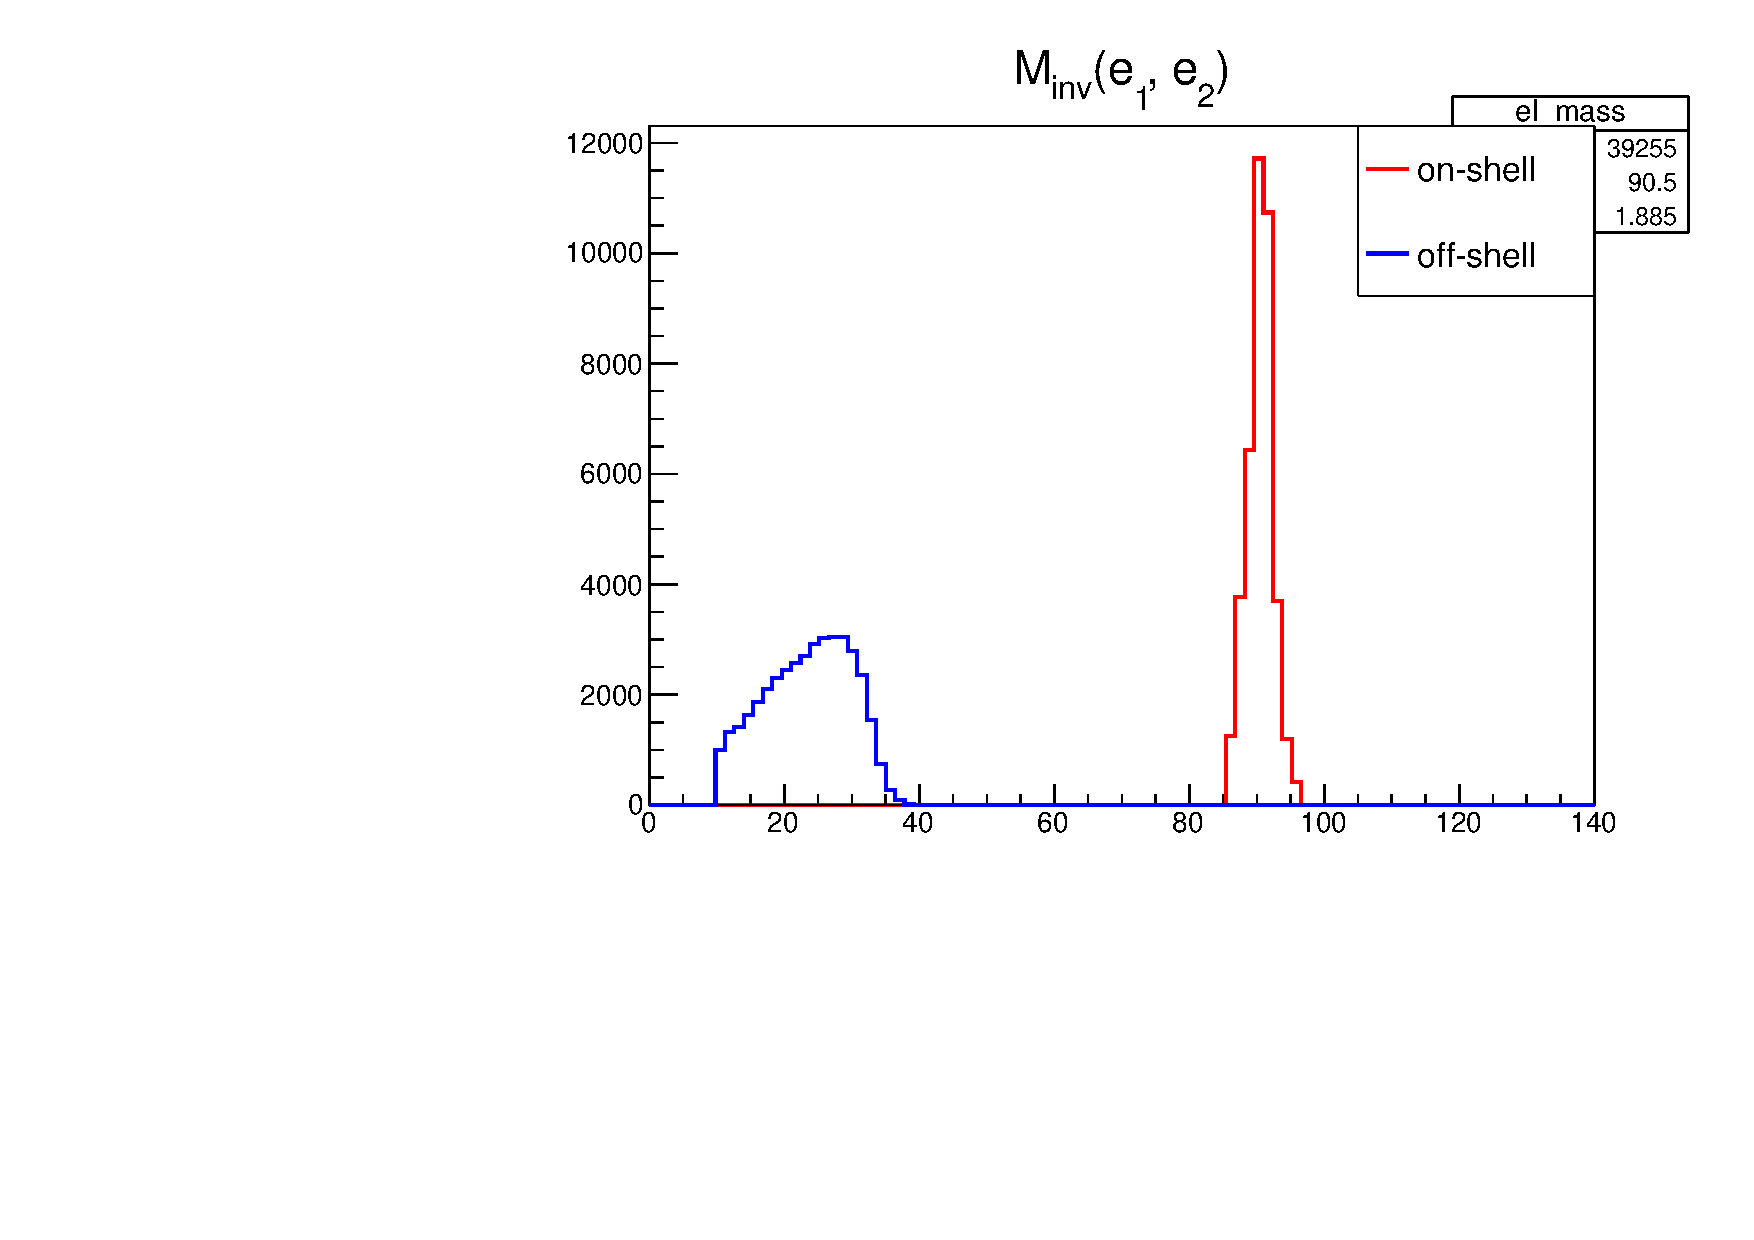
\includegraphics[width=0.7\textwidth]{figure/Mll_delphes.pdf}%Path of the figure%
%     \caption{Delphes Simulation}%Title of the figure%
%     \label{fig:mlldelphes}
% \end{figure}


\bibliographystyle{ieeetr}
\bibliography{refer}
\end{document}